% ----------------------------------------------------------------------------
% GUI
% ----------------------------------------------------------------------------

\chapter{Externals com GUI - Usando o Tcl/Tk}

O Pd permite que externals possuam interfaces gráficas mais rebuscadas que as simples
caixinhas que o mesmo desenha. Isto pode ser feito adicionando código Tcl/tk ao external.
Isto porque a GUI do próprio Pd é feita nesta linguagem.

\section{Escrevendo externals com GUI}

A primeira necessidade para implementar um external com GUI é a inclusão da biblioteca g\_canvas.h. Esta biblioteca
encontra-se disponível em \footnote{http://www.koders.com/c/fid97160440CD236854358462C336536646E0933C46.aspx} e nela estarão
as funcionalidades necessárias para que o Pd desenhe nossas GUI. Veja que não queremos alterar a GUI do Pd mas
apenas fazer uma GUI para o external. Isto significa que teremos o cuidade de pedir ao Pd que desenhe nossa GUI.

O segundo passo é definirmos uma variável para armazenar o comportamento do nosso objeto (Veja o exemplo 14).

\begin{lstlisting}
t_widgetbehavior widgetbehavior; // This represents the external GUI
\end{lstlisting}

Nesta variável teremos as funções definidas para o que acontece com nosso objeto gráfico. Isto deve ser 
feito no método setup do objeto.

\begin{lstlisting}
void example14_setup(void) {
    example14_class = class_new(gensym("example14"),
            (t_newmethod) example14_new, // Constructor
            (t_method) example14_destroy, // Destructor
            sizeof (t_example14),
	    CLASS_DEFAULT,
	    A_GIMME, // Allows various parameters
            0); // LAST argument is ALWAYS zero

    // The external GUI rectangle definition
    widgetbehavior.w_getrectfn = my_getrect;
    //How to make ir visible / invisible
    widgetbehavior.w_visfn= my_vis;
    //what to do whe moved
    widgetbehavior.w_displacefn= my_displace;
    // What to do when selected
    widgetbehavior.w_selectfn= my_select;
    // What to do when active
    widgetbehavior.w_activatefn = my_activate;
    // What to do when deleted
    widgetbehavior.w_deletefn = my_delete;
    // What to do when clicked
    widgetbehavior.w_clickfn = my_click;

    // What about object properties?
    class_setpropertiesfn(example14_class, my_properties);
    // How to save its properties with the patch?
    class_setsavefn(example14_class, my_save);

    //Associate the widgetbehavior with the class
    class_setwidget(example14_class, &widgetbehavior);

}
\end{lstlisting}

Além de definir as funções callback da GUI é necessário associar o widgetbehavior a classe. Uma vez que isto
for feito, o Pd não mais irá renderizar a famosa caixinha. A partir disto a responsabilidade de renderizar a 
GUI passa a ser do programador.

Vamos ver as funções criadas para desenhar uma GUI.

\begin{lstlisting}
// THE BOUNDING RECTANGLE
static void my_getrect(t_gobj *z, t_glist *glist, int *xp1, int *yp1, int *xp2, int *yp2){
	// This function is always called. 
	// Better do not put a post here...
	// post("GETRECT");
	t_example14 *x = (t_example14 *)z;
 	*xp1 = x->x_obj.te_xpix;
 	*yp1 = x->x_obj.te_ypix;
 	*xp2 = x->x_obj.te_xpix + 30;
 	*yp2 = x->x_obj.te_ypix + 50;
}
\end{lstlisting}

Esta função recebe ponteiros para inteiros que deverão ser apontados para os valores que queremos definir como
o retângulo do nosso objeto. Veja que isto não é necessariamente o tamanho do retângulo do objeto gráfico mas aonde o mesmo
poderá ser clicado na tela. Um exemplo disto é o comentário do Pd. Apesar do mesmo as vezes ficar maior, sua área 
clicável é sempre um quadradinho na esquerda. Isto significa que nem sempre a representação gráfica da área do objeto
é a mesma da sua área de desenho.

\begin{lstlisting}
// MAKE VISIBLE OR INVISIBLE
static void my_vis(t_gobj *z, t_glist *glist, int vis){
	t_example14 *x = (t_example14 *)z;

	// takes the Canvas to draw a GUI
	t_canvas * canvas = glist_getcanvas(glist);

	if(vis){ // VISIBLE
	post("VISIBLE");

        sys_vgui(".x%lx.c create rectangle %d %d %d %d -tags %xrr -fill #FF0000\n",
		glist_getcanvas(glist),
		x->x_obj.te_xpix,
		x->x_obj.te_ypix,
		x->x_obj.te_xpix + 70,
		x->x_obj.te_ypix + 50,
		x
		);
       sys_vgui(".x%x.c create text %d %d -text {example14} -anchor w  -tags %xlb\n",
                canvas,
		x->x_obj.te_xpix + 2,
		x->x_obj.te_ypix + 12,
		x);
	}else{ // INVISIBLE
		post("INVISIBLE");
		sys_vgui(".x%x.c delete %xrr\n",canvas, x);
		sys_vgui(".x%x.c delete %xlb\n",canvas, x);
	}
//	canvas_fixlinesfor(glist, (t_text *)x);
}\end{lstlisting}

Deixar o objeto visível ou invisível significa pedir a GUI do Pd que desenhe ou apague um desenho.
Neste caso nosso desenho é um retângulo vermelho. Usamos o nome da própria instância como nome do
objeto Tk para evitar que sobrescrevamos o nome de algum outro componente gráfico do Pd. Também desenhamos
um texto com o nome do objeto pois o Pd não fará isto. Caso nosso objeto se torne invisível, temos de
remover ambos do canvas.

\begin{lstlisting}
// WHAT TO DO IF SELECTED?
static void my_select(t_gobj *z, t_glist *glist, int state){
 	t_example14 *x = (t_example14 *)z;
 	if (state) {
	post("SELECTED");
        sys_vgui(".x%x.c create rectangle %d %d %d %d -tags %xSEL -outline blue\n",
		glist_getcanvas(glist),
		x->x_obj.te_xpix,
		x->x_obj.te_ypix,
		x->x_obj.te_xpix + 70,
		x->x_obj.te_ypix + 50,
		x
		);
	}else {
	post("DESELECTED");
 	sys_vgui(".x%x.c delete %xSEL\n",glist_getcanvas(glist), x);
	}
}
\end{lstlisting}

O que acontece quando um objeto do Pd é selecionado? Ele ganha um contorno azul. O que acontece
quando nosso objeto é selecionado? Nada. Por isto desenhamos aqui um contorno azul. Quando ele
é deselecionado, removemos o contorno azul.

\begin{lstlisting}
// DISPLACE IT
void my_displace(t_gobj *z, t_glist *glist,int dx, int dy){
	post("MOVED");
	t_canvas * canvas = glist_getcanvas(glist);
	t_example14 *x = (t_example14 *)z;
	x->x_obj.te_xpix += dx; // x movement
	x->x_obj.te_ypix += dy; // y movement

        sys_vgui(".x%lx.c coords %xSEL %d %d %d %d \n", //MOVE O SELECIONADO
		canvas,
		x,
		x->x_obj.te_xpix,
		x->x_obj.te_ypix,
		x->x_obj.te_xpix + 70,
		x->x_obj.te_ypix + 50
		);
        sys_vgui(".x%x.c coords %xrr %d %d %d %d\n",canvas,x,x->x_obj.te_xpix,x->x_obj.te_ypix,x->x_obj.te_xpix + 70,x->x_obj.te_ypix + 50);
        sys_vgui(".x%x.c coords %xlb %d %d \n",canvas,x,x->x_obj.te_xpix + 2, x->x_obj.te_ypix + 12);

	canvas_fixlinesfor(glist, (t_text *)x);
}
\end{lstlisting}

O que fazer quando movemos um objeto. Aqui será necessário mover todos os objetos pois não temos um
container que possui todos os objetos. Inclusive é necessário mover o contorno azul que desenhamos
quando o mesmo se tornou selecionado.

\begin{lstlisting}
// What to do if activated?
static void my_activate(t_gobj *x, struct _glist *glist, int state){
	post("Activated");
}
\end{lstlisting}

O método será executado quando um objeto se tornar ativo.

\begin{lstlisting}
static int my_click(t_gobj *z, struct _glist *glist, int xpix, int ypix, int shift, int alt, int dbl, int doit){
	post("Clicked xpix:%d ypix:%d shift:%d alt:%d dbl:%d doit:%d", xpix,ypix, shift, alt, dbl, doit);
	return 0;
}
\end{lstlisting}

O método click é retornado com qualquer evento do mouse. Caso ele seja clicado, o mesmo receberá o valor 1 no parâmetro doit.
Vale lembrar que este método só será executado quando o Pd não estiver no modo de edição.

\begin{lstlisting}
static void my_delete(t_gobj *z, t_glist *glist){
	t_text *x = (t_text *)z;
	canvas_deletelinesfor(glist_getcanvas(glist), x);
	post("Object deleted!");
} 
\end{lstlisting}

Este método será o destrutor da GUI.

\begin{lstlisting}
void my_save(t_gobj *c, t_binbuf *b){
	post("SAVE");
}
\end{lstlisting}

Quando salvamos o \patch pode ser necessário armazenar parâmetros para recuperar nosso external
como GUI na mesma situação. Este método recebe um buffer aonde poderá armazenar dados que serão
devolvidos quando o mesmo for recriado. Note que isto não está associado com a GUI mas com a classe.

\todo{Nunca implementei Salvar. Parece legal...}


\begin{lstlisting}
void my_properties(t_gobj *c, t_glist *list){
	post("PROPERTIES");
}
\end{lstlisting}

Caso o usuário pressione o botão contrário ele pode alterar as propriedades do objeto. Este método
permite definir a lista de propriedades que o objeto aceita. Note que isto não está associado com a GUI
mas com a classe.

\todo{Ainda não implementei propriedades.}

Caso nosso objeto tenha sido criado corretamente, ele ficará como a seguir
\begin{figure}[h!]
	\centering
	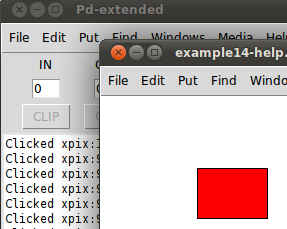
\includegraphics[width=0.7\textwidth]{example14}
	\caption{Adicionando GUI tk.}
\end{figure}

Note que este objeto foi definido em sua criação como um CLASS\_DEFAULT, o que implica que o mesmo possui
um inlet. Este inlet existe e está funcionando e aceitando conexões de outros objetos, mensagens e números.
Só não aceita conexões DSP pois as mesmas não foram definidas para este objeto. 
Mesmo assim o Pure Data não irá desenhá-lo pois precisamos definir tudo na GUI. Caso queira um
retângulo em cima para mostrar ao usuário que temos um inlet, temos que desenhá-lo, movê-lo quando necessário e 
também apagá-lo quando o objeto se tornar invisível.

\section{Adicionando componentes gráficos}

O Objeto Tk que o Pd nos disponibiliza é um canvas. Um canvas é, em princípio, uma tela de pintura. Em um canvas 
podemos adicionar linhas, ovals, pontos, textos, retângulos e janelas. É por se tratar de um canvas e não de uma
janela que não temos o conceito de um container para os objetos. Desta maneira, para adicionarmos um componente 
como um botão ou um slider, é necessário adicionarmos uma janela ao canvas para que a mesma abrigue este componente gráfico.
Há vários componentes gráficos que podem ser adicionados em um external. Vejamos um exemplo (exemplo 15).

\begin{lstlisting}
// MAKE VISIBLE OR INVISIBLE
static void my_vis(t_gobj *z, t_glist *glist, int vis){
	t_example15 *x = (t_example15 *)z;
	t_canvas * canvas = glist_getcanvas(glist);

	if(vis){ // VISIBLE
	// Define the tk/tcl commands / functions
	sys_vgui("proc do_something {} {\n set name [.x%x.c.s%xtx get]\n puts \"OIA: $name\" \n}\n",canvas,x);
	sys_vgui("proc do_otherthing {val} {\n set name [.x%x.c.s%xtx get]\n puts \"OIA: $name\" \n}\n",canvas,x);
    	// The text field
	sys_vgui("entry .x%x.c.s%xtx -width 12 -bg yellow \n", canvas,x);
	// The button
	sys_vgui("button .x%x.c.s%xbb -text {click} -command do_something\n", canvas,x);
	// The radio button	
	sys_vgui("radiobutton .x%x.c.s%xrb -value 1 -command do_something\n", canvas,x);
	// The h slider
	sys_vgui("scale .x%x.c.s%xsb -orient horizontal -command do_otherthing \n", canvas,x);
	// A checkbutton
	sys_vgui("checkbutton .x%x.c.s%xcb -foreground blue -background yellow -command do_something\n", canvas,x);
	// The red rectangle
        sys_vgui(".x%lx.c create rectangle %d %d %d %d -tags %xrr -fill #FF0000\n",
		glist_getcanvas(glist),
		x->x_obj.te_xpix,
		x->x_obj.te_ypix,
		x->x_obj.te_xpix + 170,
		x->x_obj.te_ypix + 150,
		x
		);
	// A window to the button (bb)
	sys_vgui(".x%x.c create window %d %d -anchor nw -window .x%x.c.s%xbb -tags %xbb\n",
		canvas,
		x->x_obj.te_xpix + 70,
		x->x_obj.te_ypix + 120,
		canvas,
		x,
		x);
	// A window to the radiobutton
	sys_vgui(".x%x.c create window %d %d -anchor nw -window .x%x.c.s%xrb -tags %xrb\n",
		canvas,
		x->x_obj.te_xpix + 70,
		x->x_obj.te_ypix,
		canvas,
		x,
		x);
	// A window to the combo box 
	sys_vgui(".x%x.c create window %d %d -anchor nw -window .x%x.c.s%xcb -tags %xcb\n",
		canvas,
		x->x_obj.te_xpix  + 100,
		x->x_obj.te_ypix,
		canvas,
		x,
		x);
	// A window to the slider button
	sys_vgui(".x%x.c create window %d %d -anchor nw -window .x%x.c.s%xsb -tags %xsb\n",
		canvas,
		x->x_obj.te_xpix,
		x->x_obj.te_ypix + 80,
		canvas,
		x,
		x);
	// A window to the text
	sys_vgui(".x%x.c create window %d %d -anchor nw -window .x%x.c.s%xtx -tags %xtx\n",
		canvas,
		x->x_obj.te_xpix,
		x->x_obj.te_ypix + 60,
		canvas,
		x,
		x);
	// a label field
       sys_vgui(".x%x.c create text %d %d -text {example15~} -anchor w  -tags %xlb\n",
                canvas,
		x->x_obj.te_xpix,
		x->x_obj.te_ypix + 40,
		x);

	}else{ // INVISIBLE
		sys_vgui(".x%x.c delete %xbb\n",canvas, x);
		sys_vgui(".x%x.c delete %xcb\n",canvas, x);
		sys_vgui(".x%x.c delete %xrb\n",canvas, x);
		sys_vgui(".x%x.c delete %xsb\n",canvas, x);
		sys_vgui(".x%x.c delete %xrr\n",canvas, x);
		sys_vgui(".x%x.c delete %xlb\n",canvas, x);
		sys_vgui(".x%x.c delete %xtx\n",canvas, x);
	}
}
\end{lstlisting}

Criamos os componentes gráficos e pedimos ao canvas para criar uma janela para que a mesma abrigue o componente.
Assim, na hora de remover podemos remover apenas a janela. O mesmo ocorre na hora de mover.
Note que além de adicionarmos componentes gráficos associamos eles a um comando. Este será nosso próximo tópico.

\begin{lstlisting}
void my_displace(t_gobj *z, t_glist *glist,int dx, int dy){
	t_canvas * canvas = glist_getcanvas(glist);
	t_example15 *x = (t_example15 *)z;
	x->x_obj.te_xpix += dx;
	x->x_obj.te_ypix += dy;

        sys_vgui(".x%lx.c coords %xSEL %d %d %d %d \n", //MOVE O SELECIONADO
		glist_getcanvas(glist),
		x,
		x->x_obj.te_xpix,
		x->x_obj.te_ypix,
		x->x_obj.te_xpix + 170,
		x->x_obj.te_ypix + 150
		);
        sys_vgui(".x%x.c coords %xrr %d %d %d %d\n",canvas,x,x->x_obj.te_xpix,x->x_obj.te_ypix,x->x_obj.te_xpix + 170,x->x_obj.te_ypix + 150);
        sys_vgui(".x%x.c coords %xbb %d %d \n",canvas,x,x->x_obj.te_xpix,x->x_obj.te_ypix);
        sys_vgui(".x%x.c coords %xcb %d %d \n",canvas,x,x->x_obj.te_xpix + 30,x->x_obj.te_ypix);
        sys_vgui(".x%x.c coords %xsb %d %d \n",canvas,x,x->x_obj.te_xpix,x->x_obj.te_ypix + 80);
        sys_vgui(".x%x.c coords %xtx %d %d \n",canvas,x,x->x_obj.te_xpix,x->x_obj.te_ypix + 120);
        sys_vgui(".x%x.c coords %xrb %d %d \n",canvas,x,x->x_obj.te_xpix + 60,x->x_obj.te_ypix);
        sys_vgui(".x%x.c coords %xlb %d %d \n",canvas,x,x->x_obj.te_xpix,x->x_obj.te_ypix + 40);

	canvas_fixlinesfor(glist, (t_text *)x);
}
\end{lstlisting}

\section{Adicionando comandos}

Os comandos dos nossos componentes gráficos podem ser recebidos e interagirem com o external assim como o
external consegue alterar os valores da GUI dependendo do que recebe em seus inlets. Veja o exemplo 21.

Para este exemplo, definimos na criação da classe no método setup() os métodos de retorno de nossa GUI.

\begin{lstlisting}
// depois associaremos estes "tipos" de mensagem aos inlets 2 e 3
    class_addmethod(example21_class, (t_method)example21_alfa,  gensym("alfa"), A_DEFFLOAT,0); 
    class_addmethod(example21_class, (t_method)example21_beta,  gensym("beta"), A_DEFFLOAT,0); 
// metodo do botao ok
    class_addmethod(example21_class, (t_method)example21_btok,gensym("btok"), A_DEFSYMBOL,0); 
\end{lstlisting}

No método vis da GUI, criamos comandos.

\begin{lstlisting}
	    sys_vgui("proc slide_alfa {val} {\n pd [concat example21%x alfa $val \\;]\n}\n",x);
	    sys_vgui("proc slide_beta {val} {\n pd [concat example21%x beta $val \\;]\n}\n",x);
	    sys_vgui("proc botao_ok {} {\n set name [.x%x.c.s%xtx get]\n pd [concat example21%x btok $name \\;]\n}\n",x->canvas,x,x);
	    sys_vgui("proc botao_file_chooser {} {\n\
						   set filename [tk_getOpenFile]\n\
						  .x%x.c.s%xtx delete 0 end \n\
						  .x%x.c.s%xtx insert end $filename \n}\n",x->canvas,x,x->canvas,x);

	(...)
	sys_vgui("entry .x%x.c.s%xtx -width 25 -bg white -textvariable \"teste\" \n", x->canvas,x);
	sys_vgui("button .x%x.c.s%xbfc -text {...} -command botao_file_chooser\n", x->canvas,x);
	sys_vgui("scale .x%x.c.s%xsb1 -length 250 -resolution 0.01 -from 0.5 -to 2 -orient horizontal -command slide_alfa \n", x->canvas,x);
	sys_vgui("scale .x%x.c.s%xsb2 -length 250 -resolution 0.01 -from 0.5 -to 2 -orient horizontal -command slide_beta \n", x->canvas,x);
	sys_vgui("button .x%x.c.s%xbt -text {start} -command botao_ok\n", x->canvas,x);
	(...)
\end{lstlisting}

Os comandos alfa, beta e btok serão executados pelo objeto pd. Desta forma pedimos ao pd que, ao chamarmos este método o mesmo chame
a função associada a este symbolo anteriormente. Os objetos criados usarão estes comandos para suas ações.
Note que no caso do filechooser, o comando irá associar o caminho do arquivo escolhido com nosso campo text e tudo isto será feito
diretamente no Tk.

Então basta criarmos as funções associadas:

\begin{lstlisting}
static void example21_btok(t_example21* x, t_symbol * file_name){
    x->file_name = file_name->s_name;
    example21_bang(x); 
}

// Metodo para definir o nome do arquivo com retorno para a GUI
void example21_set_file_name(t_example21 *x, char * file_name){
    sys_vgui(".x%x.c.s%xtx delete 0 end \n", x->canvas, x);
    sys_vgui(".x%x.c.s%xtx insert end %s\n", x->canvas, x , file_name);
    x->file_name = file_name;
    // DO SOMETHING
}

void example21_alfa(t_example21 *x, t_floatarg f){
    if( f >= 2) f = 2;
    if( f <= 0.5) f = 0.5; 
    sys_vgui(".x%x.c.s%xsb1 set %f\n",x->canvas,x,f);
    x->alfa = f;
}

void example21_beta(t_example21 *x, t_floatarg f){
    if( f >= 2) f = 2;
    if( f <= 0.5) f = 0.5; 
    sys_vgui(".x%x.c.s%xsb2 set %f\n",x->canvas,x,f);
    x->beta = f;
}
\end{lstlisting}

O resultado é visto a seguir.

\begin{figure}[h!]
	\centering
	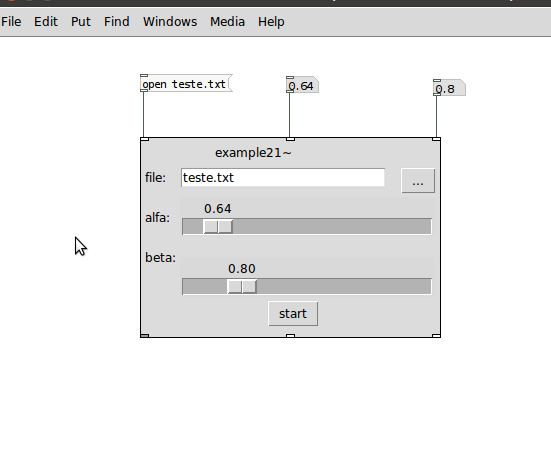
\includegraphics[width=0.7\textwidth]{example21}
	\caption{External com GUI e comandos}
\end{figure}


